\subsection{Comparison to the {\it Planck} catalog of tSZ sources}
The overall integrated Compton parameter for \mbox{RX~J1347.5-1145} can be compared to the {\it Planck} satellite measurement, as reported in the {\it Planck} catalog of tSZ sources \citep{Planck_survey}. For each detection, the {\it Planck} catalog provides the two-dimensional  $\theta_s$~--~$Y_{5r_{500}}$ probability distribution. The parameter $\theta_s$ is again the characteristic radius of Eq. \ref{eq:gNFW}, and $Y_{5r_{500}}$ is the integrated Compton parameter within a radius equal to 5$\times r_{500}$, therefore, assumed to be the total flux. The catalog also contains the slopes of the gNFW pressure profile used by the detection pipeline, which allows us to compute the $Y_{\theta_{\mathrm{max}}}$ / $Y_{5R_{500}}$ ratio, so to extrapolate the {\it Planck} flux ($Y_{5R_{500}}$) to the integrated signal at any cluster centric distance ($Y_{\theta_{\mathrm{max}}}$). To compare our result to {\it Planck} data, we have explored two different methodologies:

\begin{itemize}
\item {We fixed $\theta_s$ to its maximum likelihood value, obtaining $Y_{5R_{500}}~=~(2.17~\pm~0.36)~\times~10^{-3}$~arcmin$^2$ for \mbox{RX~J1347.5-1145}. Then, the $Y_{\theta_{\mathrm{max}}}$ / $Y_{5R_{500}}$ ratio returns $Y^{Planck}_{\theta_{\mathrm{max}}}$~=~$(1.78 \pm 0.30) \times 10^{-3}$~arcmin$^2$ for $\theta_{\mathrm{max}} = 2$~arcmin, which agrees with the {\it NIKA} value, $Y^{total}_{\theta_{\mathrm{max}}}$~=~$(1.73~\pm~0.45)~\times~10^{-3}$~arcmin$^2$.  
\item The {\it Planck} tSZ angular size ($\theta_s$) -- flux ($Y_{5r_{500}}$) degeneracy can also be broken by fixing $r_{500}$ to its \mbox{X-ray} derived value without changing the other pressure profile parameters. This includes $c_{500}$ (which is kept equal to 1.1733; the value given by \citealp{arnaud_2010}). This is what \citealp{Planck_survey} uses, when recovering the integrated tSZ signal within the \mbox{X-ray} size. Following this approach, we obtain $Y^{Planck}_{\theta_{\mathrm{max}}}$~=~$(1.23~\pm~0.21)~\times~10^{-3}$~arcmin$^2$ for $\theta_{\mathrm{max}}~=~2$~arcmin. This value is still consistent with the {\it NIKA} flux, although weaker. The latter can be understood if we consider that the \mbox{X-ray} derived $r_{500}$~=~1.42~Mpc~$\equiv~\theta_{500}$=~3.94~arcmin \citep[{\it MCXC},][]{MCXC} is much larger than the reliable radial extent of the {\it NIKA} map. The $r_{500}$ that can be deduced from the {\it NIKA} $\theta_s$ parameter is, by contrast, smaller. However, we expect the two integrated Compton parameters to converge when we move to larger $\theta_{\mathrm{max}}$. Indeed, when pushing the integration up to $\theta_{\mathrm{max}} = 2.5$~arcmin (by extrapolating the best-fit model of the relaxed region to angular distances not directly probed through our observations and assuming that the contribution due to the shock is negligible at scales larger than $\sim$ 2~arcmin), we obtain $Y^{Planck}_{\theta_{\mathrm{max}}}$~=~$(1.52~\pm~0.26)~\times~10^{-3}$~arcmin$^2$ versus $(1.77~\pm~0.45)~\times~10^{-3}$~arcmin$^2$ for {\it NIKA}. Alternatively, the larger {\it NIKA} flux can also be explained by relaxing the hypothesis of a constant $c_{500}$. The different sensitivities of {\it Planck}+{\it MCXC} and {\it NIKA} to the signal distribution could lead to differences in the recovered flux distribution. With $r_{500}$ fixed to its \mbox{X-ray} value, a larger value of $c_{500}$ implies a smaller value of  $\theta_s$ and, therefore, that a larger fraction of the total tSZ flux is located within the innermost regions. In this case, we would have a better consistency between  the {\it Planck}+{\it MCXC} and the {\it NIKA} integrated Compton parameter, even at smaller cluster-centric distances. Since the value of $c_{500}=1.1733$ has been obtained on an average (universal) profile~\citep{arnaud_2010} and \mbox{RX~J1347.5-1145} is known to have a very peaked morphology compared to other clusters, this hypothesis is likely to be correct: the inner slope parameter $\gamma$ being fixed, $c_{500}$ can typically vary from $\sim$ 0 to $\sim$ 5 between clusters~\citep{planck_pp}.}
\end{itemize}

From the comparison to the {\it Planck} data, we can conclude that {\it NIKA} is able to recover most of the tSZ signal, despite the large angular scale cutoff (above 3~arcmin). This is consistent with what was found in the simulations in Sect.~\ref{sec:valid_pipe_simu} and in particular for the compact cluster case, which is very similar to the {\it NIKA} \mbox{RX~J1347.5-1145} observations regarding the tSZ flux and angular extension. From this, we can convey that {\it Planck} and {\it NIKA} are complementary. This will be even more interesting and easily exploitable with the larger field of view (6.5~arcmin) that the {\it NIKA2} camera will reach.

\subsection{Comparison to {\it DIABOLO} tSZ observations}
\label{sec:comp_sz}
In Fig.~\ref{fig:NIKAvsDIABOLO}, we present the comparison between {\it DIABOLO} and the {\it NIKA} results on \mbox{RX~J1347.5-1145}. {\it DIABOLO} \citep{pointecouteau_1999, pointecouteau_2001} was a bolometric camera that observed \mbox{RX~J1347.5-1145} at the IRAM 30-meter telescope using a dual-band instrument at frequencies corresponding to the {\it NIKA} bands: 140 and 250~GHz. The resolution of {\it DIABOLO} was 22~arcsec at 140~GHz. The data reduction and the instrumental similarities with {\it NIKA} make it a first choice for a direct comparison.

The left panel shows the tSZ {\it NIKA} map with {\it DIABOLO} contours overplotted in red with levels of -1, -3, -5, and -7 mJy/beam (radio source not subtracted in both maps).  We can see that the tSZ maxima and the external part of the cluster match within error bars. The overall amplitude of the signal is slightly higher for {\it NIKA} data than for {\it DIABOLO}. However, this difference is not significant once we account for the  systematic uncertainties given in Table~\ref{tab:table_err}. The right panel of Fig.~\ref{fig:NIKAvsDIABOLO} compares the cluster pressure profile (radio source subtracted and X-rays centered) measured with both instruments. The two profiles are compatible within error bars over the whole radial range, even though {\it NIKA} seems to detect more signal in the inner part of the cluster. The reduced $\chi^2$ associated to the profile difference, which is computed up to a radius of 2.5~arcmin, is equal to 2.35. However, since this does not account for calibration uncertainties, we also give the reduced $\chi^2$ after cross calibrating the two profiles: we obtain $\chi^2 = 1.32$ with a cross-calibration factor of 1.09, which is compatible with our calibration error estimate. In both cases, the tSZ maximum is not located at the \mbox{X-ray} center, in contrast to interferometric {\it CARMA} measurement, but agrees with other single-dish observations.

	\begin{figure*}
	\centering
	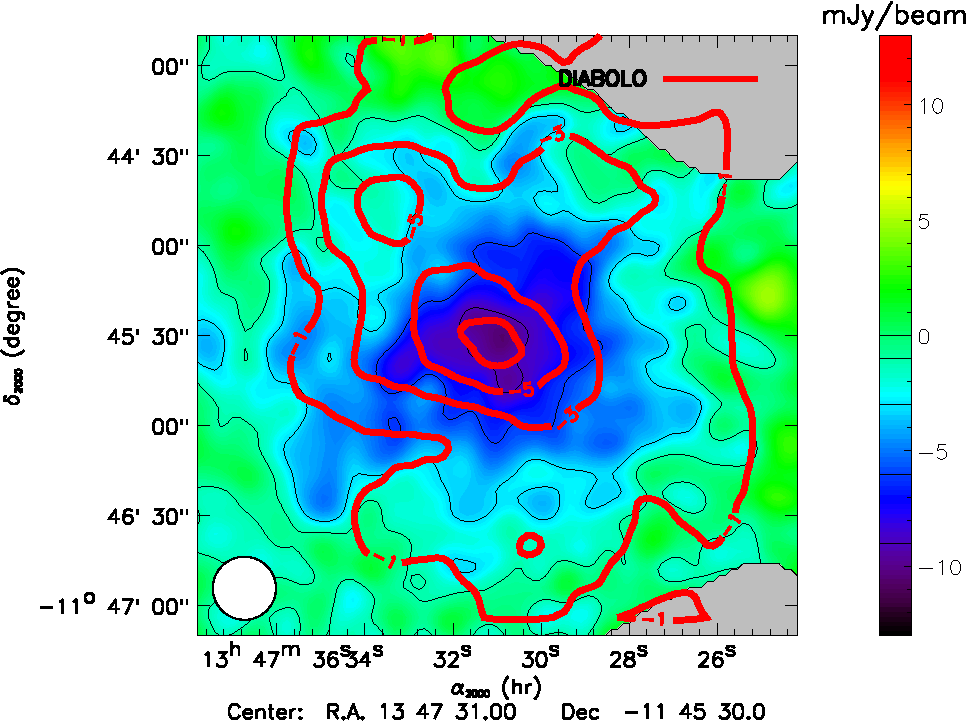
\includegraphics[width=0.45\textwidth]{Figure/RXJ1347-1145_NIKAvsDIABOLO_PS_subtracted}
	\hspace*{0.5cm}
	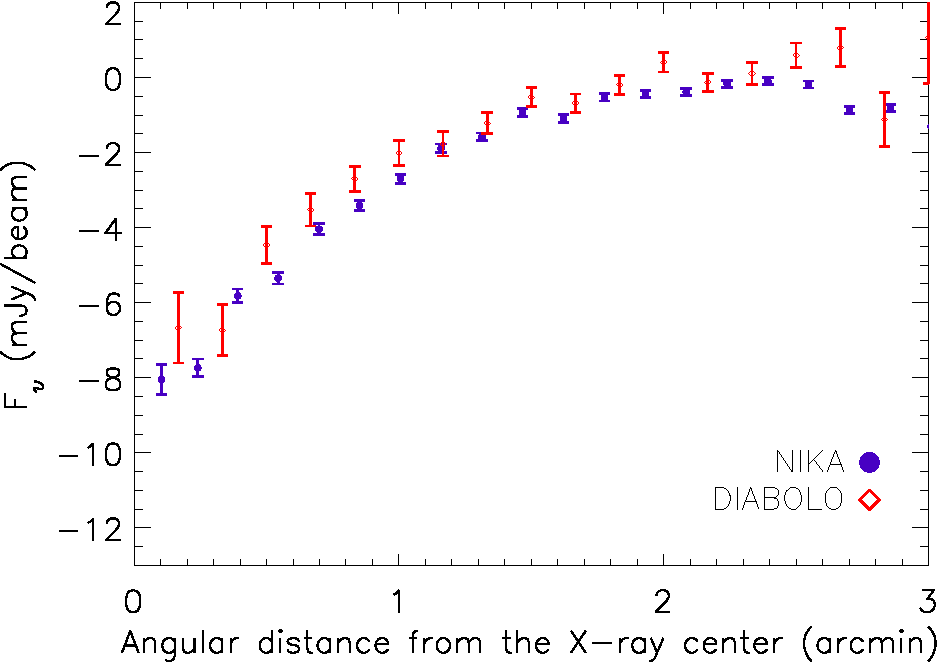
\includegraphics[width=0.45\textwidth]{Figure/profile_DIABOLO_vs_NIKA}
	\caption{Comparison of \mbox{RX~J1347.5-1145} tSZ maps by {\it DIABOLO} and {\it NIKA} in mJy/beam. Left: {\it NIKA} tSZ map with {\it DIABOLO} contours in red at -1, -3, -5, and -7 mJy/beam. Right: Flux radial profile as measured by {\it NIKA} (purple dots) and {\it DIABOLO} (red diamonds).}
        \label{fig:NIKAvsDIABOLO}
	\end{figure*}

\subsection{Comparison to {\it XMM} and {\it Chandra} \mbox{X-ray} observations}
\label{sec:comp_x}
The {\it XMM} data \citep{gitti_2004} have been used to compute a photon count (exposure corrected) map of \mbox{RX~J1347.5-1145} that we compare to the {\it NIKA} tSZ observations. As seen in Fig.~\ref{fig:NIKAvsXray}, the tSZ peak does not coincide with the \mbox{X-ray} center. The object \mbox{RX~J1347.5-1145} gives a striking example of the power of tSZ data and how it complements \mbox{X-ray}. Moreover, the mismatch between the tSZ and \mbox{X-ray} center gives valuable information on the gas physics at play in the ICM.

The higher resolution of the {\it Chandra} \mbox{X-ray} data has been used for cluster simulation purposes. In particular, the work of \cite{Barbara} uses the publicly available, \mbox{X-ray} derived, pressure profiles of the ACCEPT (Archive of {\it Chandra} Cluster Entropy Profile Tables) clusters \citep{Cavagnolo2009} to constrain the $P_0 $, $r_{\mathrm{s}}$, and $\gamma$ parameters of the gNFW pressure profile (Eq.~\ref{eq:gNFW}). The best-fitting values for \mbox{RX~J1347.5-1145} (Table~\ref{tab:table_clusters}) have been used in the present work to simulate the expected tSZ signal, as explained in Sect.~\ref{sec:sz_simu}. Once processed through the pipeline, the expected profile is compared to the {\it NIKA} best-fit profile, excluding the shocked area (see Sect.~\ref{sec:mcmc}) on the right panel of Fig.~\ref{fig:NIKAvsXray}. The {\it NIKA} best-fit profile and the \mbox{X-ray} model are both given with the 1$\sigma$ error envelope. The error on the {\it NIKA} profile only accounts for statistical uncertainties by sampling the 1$\sigma$ contour of the likelihood of Fig.~\ref{fig:likelihood}. The systematic errors (see Eq.~\ref{eq:best_fit_nika}) are not shown and would result in an overall multiplicative factor on the amplitude ($P_0$) and on the angular scale ($\theta_s$). We choose to include only the error on the parameter $P_0$ (Table~\ref{tab:table_clusters}) for the \mbox{X-ray} model, since it is highly degenerated with $\theta_s$ and $\gamma$. In addition to the \mbox{X-ray} systematic uncertainties, the associated systematic error, which is not included in Fig.~\ref{fig:NIKAvsXray}, arises mainly from the unit conversion coefficient (Jansky per beam to Compton parameter: $y=10^{-3} \equiv 11.8 \pm 1.2$ mJy/beam). It has a similar effect as the error on the $P_0$ {\it NIKA} best-fit value. The two profiles agrees within systematic and statistical uncertainties. 
	\begin{figure*}
	\centering
	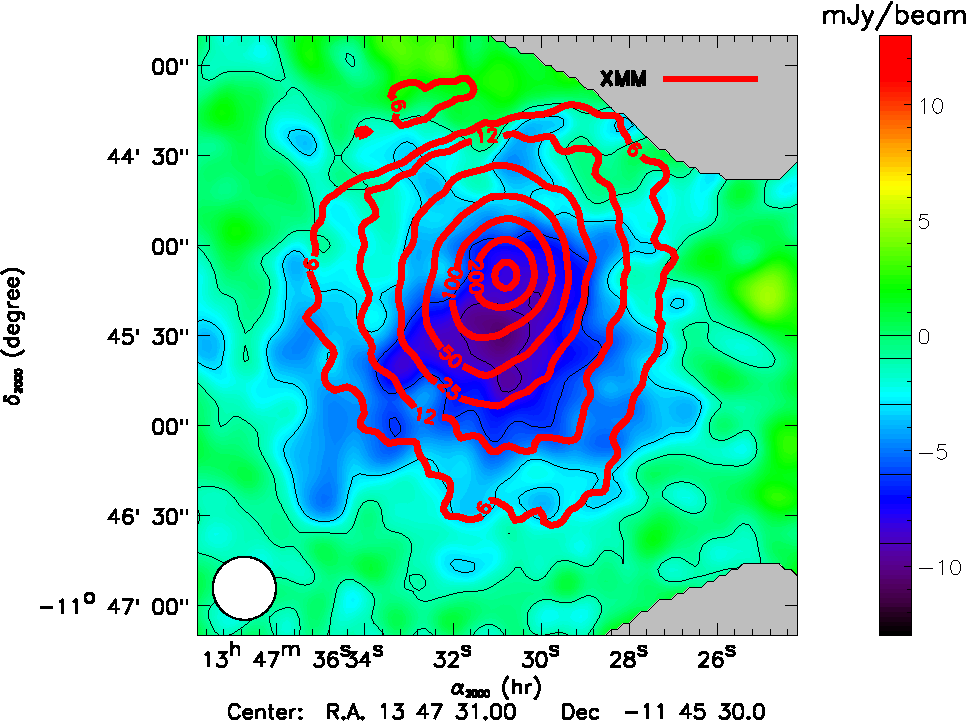
\includegraphics[width=0.45\textwidth]{Figure/RXJ1347-1145_NIKAvsXMM_PS_subtracted}
	\hspace*{0.5cm}
	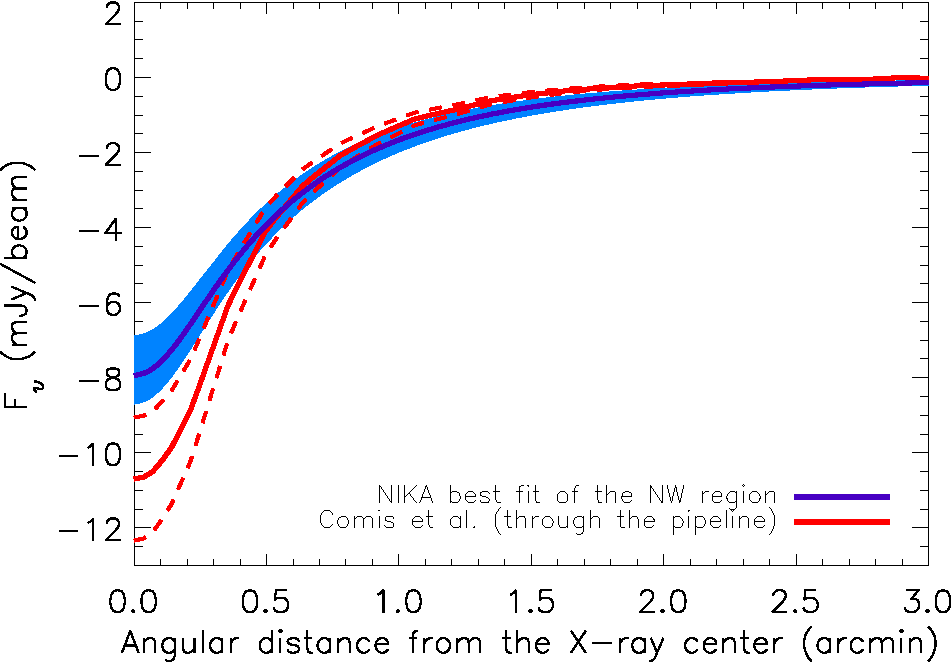
\includegraphics[width=0.45\textwidth]{Figure/NIKA_VS_Barbara}
	\caption{Left: Comparison between the \mbox{RX~J1347.5-1145} {\it NIKA} tSZ map and the {\it XMM} \mbox{X-ray} data \citep[see the work of ][]{gitti_2004,gitti_2005,gitti_2007}. The {\it XMM} map has been smoothed with a 5~arcsec Gaussian filter. The red \mbox{X-ray} contours are in photon counts and correspond to 6 12, 25, 50, 100, 200, and 400. Right: Comparison between the best-fit radial tSZ profile of the {\it NIKA} map, excluding the shock area (see Sect.~\ref{sec:mcmc}) and the profile derived from {\it Chandra}'s data by~\cite{Barbara}, which is processed through the {\it NIKA} data reduction pipeline, as discussed in Sect.~\ref{sec:TOI_ana}. The {\it NIKA} best-fit profile is given in purple with an associated 1$\sigma$ statistical error range filled in blue, and the \mbox{X-ray} model is given in red with the 1$\sigma$ statistical error limit, as two dashed lines. See text for more details on the errors limits.}
        \label{fig:NIKAvsXray}
	\end{figure*}

	\begin{table}
	\begin{center}
	\begin{tabular}{llccc}
	\hline
	\hline
	 $P_0 \ (\mathrm{keV/cm}^3)$ & $3.29 \pm 0.50$ \\
	 ($\alpha$, $\beta$, $\gamma$) & ($0.9$, $5.0$, $0.00 \pm 0.05$) \\
	 $r_{\mathrm{s}}$ (kpc) & $406 \pm 23$ \\
	 $\theta_{\mathrm{s}}$ (arcsec) &  $70 \pm 4$\\
	\hline
	\end{tabular}
	\end{center}
	\caption{Modeling of the pressure profile of \mbox{RX~J1347.5-1145} using the fit of {\it Chandra} data \citep{Barbara}. We note that $\alpha$ and $\beta$ have been fixed to the best-fitting values, as obtained by \cite{nagai_2007}, see \cite{mroczkowski_2009} for an errata.}
	\label{tab:table_clusters}
	\end{table}

\subsection{Comparison to other high resolution tSZ data}
\label{sec:comp_otherSZ}
We also compare the {\it NIKA} data with state-of-the-art sub-arcmin resolution data: {\it MUSTANG} \citep{mason_2010, korngut_2011} and {\it CARMA} \citep{plagge_2012} observations. Since these two instruments are in many ways different from {\it NIKA}, we limit ourselves to a qualitative comparison.

The instrument {\it MUSTANG} uses the single dish 100-meter Green Bank Telescope in Virginia, USA. It operates at 90~GHz with a 8~arcsec resolution. At 90~GHz, the central radio source of \mbox{RX~J1347.5-1145} is very bright compared to the tSZ decrement.  In the case of  {\it MUSTANG}, the removal of the atmospheric noise filters angular scales that are larger than about 60~arcsec. In that sense, the {\it NIKA} and {\it MUSTANG} are complementary. The instrument {\it MUSTANG} is able to measure the structural property of \mbox{RX~J1347.5-1145} at scales ranging from $\sim 10 - 60$~arcsec, while the {\it NIKA} map is reliable in the range of $\sim 20 - 200$~arcsec. The two instruments agree on the morphology of \mbox{RX~J1347.5-1145} at intermediate scales (the inner part of the -6 mJy contour on Fig.~\ref{fig:rxj}). The tSZ maximum coincides and the overall distribution of the tSZ signal is consistent on both observations. The excess seen in the region 2 of Fig.~5 in~\cite{mason_2010} does not show up clearly in the {\it NIKA} map. However, the spatial scales of this feature are smaller than 10~arcsec, and it is likely smoothed out by the {\it NIKA} beam.

The instrument {\it CARMA} is a multifrequency interferometer \citep{plagge_2012}. For \mbox{RX~J1347.5-1145} observations, they were made of 23 antennae of 3.5, 6.1, and 10.4 meter operating in three configurations at 31~GHz, 86~GHz, and 90~GHz for a total of 41.7 hours of unflagged on-source observation. Due to the complexity of combining the data in different configurations, the {\it CARMA} transfer function is not simple. Nevertheless, {\it CARMA} and {\it NIKA} agree well on scales greater than about 30~arcsec. At smaller scales, {\it CARMA} and {\it NIKA} disagree on the position of the tSZ peak.

\subsection{Point source contamination effects}
\label{sec:ps_sub_effect}
As mentioned above, the effect of point source contamination is an issue in single-dish observations. In this work, the radio source located near the \mbox{X-ray} center (within 3~arcsec) can affect our results. The {\it CARMA} data suggest that the flux of the source is underestimated when removed from single-dish data. Therefore, we have reprocessed the {\it NIKA} data by assuming that the source was 3$\sigma$ brighter than its nominal value ({\it i.e.}, 5.3 mJy instead of 4.4 mJy at 140~GHz). We obtain that the tSZ maximum is still located at the shock position. The difference in tSZ amplitude between the \mbox{X-ray} center and the shock is reduced but still inconsistent with {\it CARMA}, even though the discrepancy is smaller. Moving the tSZ maximum to the \mbox{X-ray} center would require a 5$\sigma$ positive shift of the flux of the radio source. The best-fit pressure profile parameters, $P_0$ and $r_{\mathrm{s}}$, are affected by less than 1$\sigma$ (statistical only) by the point source subtraction. This is consistent with what we observed in simulations (see Sect.~\ref{sec:valid_pipe_simu}). For the infrared source Z2, 20~arcsec NE from the \mbox{X-ray} center, we have tested adding a 0.64~mJy source at its position, which is the upper limit that we have estimated in Sect.~\ref{sec:2band_decor}. The changes in our results are negligible for the location of the tSZ maximum and for the $r_{\mathrm{s}}$ and $P_0$ values; they change by less than 0.6$\sigma$ (statistical only). The Z1 infrared source is located in the external part of the cluster and does not affect any of our results.

